\section{A sharp difference-area inequality for squared bodies}
\label{sec:squared}
Let $\sigma:\mathbb C\to\mathbb C$ be $\sigma(z)=z^2$. A source body means an origin-symmetric compact convex body $K$ with nonempty interior. The quotient of interest is
\[
 R(L)=\frac{\area(L-L)}{4\area(L)},\qquad L=\sigma(K).
\]
It is invariant under invertible affine maps of $L$. Chaidez--Tanny~\cite{CT2026} use squared planar codisks in their quaternionic construction of Finsler metrics. An upper bound $R(L)\leq r$ would, through their reversibilization argument, give $c_{\rm EHZ}(X)^2\leq2r\operatorname{vol}_4(X)$ for $I$-invariant convex $X\subset\mathbb R^4$.

\subsection{Complex squaring and reciprocal convexity}
Following Milman--Milman--Rotem~\cite{MMR2018}, write
\[
 M'=\{y:\langle y,n\rangle\leq h_M(n)^{-1}\ \text{for all }n\in S^1\}.
\]
Their Lemma 18 and Proposition 19 express $M'$ as the intersection, over $x\in M$, of the parabolic regions
\[
 P_x=\{y:\langle y,x\rangle\leq 1-\tfrac14|x|^2|\operatorname{proj}_{x^\perp}y|^2\},\quad P_0=\mathbb R^2.
\]
For $x=re^{i\theta}$, elementary squaring gives
\[
 P_x=\sigma(S_x),\qquad S_x=\{z:|\operatorname{Re}(e^{-i\theta/2}z)|\leq r^{-1/2}\}.
\]
Indeed, in coordinates $e^{-i\theta}y=u+iv$, both descriptions are $u\leq r^{-1}-rv^2/4$. The map $\sigma$ commutes with arbitrary intersections of centrally symmetric sets: the two square roots of a point either both belong to any such set or both fail to belong.

\begin{theorem}[Squared bodies and reciprocity]
The compact planar reciprocal bodies containing the origin in their interior are precisely the images $\sigma(K)$ of source bodies. Moreover,
\[
 (\sigma K)'=\sigma(K^\circ).
\]
\end{theorem}
\begin{proof}
Write $K$ as the intersection of its symmetric supporting strips with unit normals $n=e^{i\phi}$ and half-widths $h_K(n)$. Each strip maps to $P_{x_\phi}$, where $x_\phi=e^{2i\phi}/h_K(n)^2$. Consequently $\sigma K$ is convex. Since $n/h_K(n)$ runs over $\partial K^\circ$, the points $x_\phi$ run over $\partial\sigma(K^\circ)$. This last image is also convex by the same strip argument. The parabolic representation therefore gives
\[
 \sigma K=(\sigma(K^\circ))'.
\]
Apply the same identity to $K^\circ$ to obtain the stated conjugacy. Conversely, the parabolic representation of any reciprocal $M'$ identifies it with $\sigma(\bigcap_{x\in M}S_x)$. The intersection is centrally symmetric and convex; compactness and interior of its square imply the corresponding properties of the intersection itself.
\end{proof}
This is an identity in fixed Euclidean coordinates. Neither squaring nor reciprocity is asserted to commute with arbitrary affine maps.

\subsection{A shadow deformation reduces to endpoint caps}
For a squared body $L$, define
\[
 T_t(u,v)=(u+t\sqrt{u^2+v^2},v),\quad -1\leq t\leq1.
\]
For $|t|<1$, the body $T_t(L)$ is affine-equivalent to the square of the image of $K$ under $\operatorname{diag}(\sqrt{1+t},\sqrt{1-t})$, since
\[
 \sigma(\sqrt{1+t}\,x+i\sqrt{1-t}\,y)
 =(\operatorname{Re}\sigma z+t|\sigma z|,\sqrt{1-t^2}\operatorname{Im}\sigma z).
\]
In particular it is convex. Convexity at the endpoints follows by Hausdorff convergence.
\begin{lemma}[Endpoint reduction]
For every source body $K$, the ratio $R(\sigma K)$ is at most the larger of the ratios of the two caps $T_{\pm1}(\sigma K)$.
\end{lemma}
\begin{proof}
For $|t|<1$, $T_t$ is injective: it preserves the second coordinate and its first coordinate is strictly increasing on each horizontal line. Its Jacobian, away from the origin, is $1+tu/\sqrt{u^2+v^2}$. Thus
\[
 \area(T_tL)=A+tB,\quad A=\area(L),\quad B=\int_L\frac{u}{\sqrt{u^2+v^2}}\,du\,dv.
\]
Here $|B|<A$ since $L$ has interior. Continuity extends the formula to $t=\pm1$.
The difference bodies are
\[
 T_tL-T_tL=\conv\{w-z+t(|w|-|z|)(1,0):w,z\in L\}.
\]
They form a shadow system, so their areas $N(t)$ are convex in $t$. For completeness, intersect such a convex hull with a fixed horizontal line. Its right endpoint is the supremum of the affine functions of $t$ obtained from convex combinations of moving points whose vertical coordinates average to that line; its left endpoint is the corresponding infimum. The width is convex in $t$, and integration over the unchanged vertical projection proves area convexity. This is the planar shadow-system argument of Rogers--Shephard. Hence $N(t)$ is bounded by the affine interpolation of its endpoint values. Divide by the positive affine denominator $4(A+tB)$; the result is bounded by the larger endpoint quotient.
\end{proof}
Since $T_1(\sigma(x+iy))=(2x^2,2xy)$, the relevant caps, up to a harmless common scale, are
\[
 C_K=\{(x^2,xy):(x,y)\in K\}.
\]
The other endpoint is the same construction after interchanging source coordinates.

\subsection{Positive tent decompositions reduce to one parameter}
Normalize the horizontal projection of $K$ to $[-1,1]$ and write
\[
 K=\{(x,y):-1\leq x\leq1,\ -b(-x)\leq y\leq b(x)\},
\]
where $b$ is concave. A shear $y\mapsto y+cx$ induces the affine shear $(u,v)\mapsto(u,v+cu)$ on $C_K$. Choose $c$ so that $b(-1)=b(1)=d\geq0$. Then $b\geq d$.
The cap $C_b$ has vertical sections
\[
 -V_b(u)\leq v\leq U_b(u),\quad
 U_b(u)=\sqrt u\,b(\sqrt u),\quad V_b(u)=\sqrt u\,b(-\sqrt u),\quad 0\leq u\leq1.
\]
Its area $A(b)=\int_0^1(U_b+V_b)$ is linear in $b$. For $0\leq s\leq1$, put
\[
 H_+(b,s)=\max_{0\leq u\leq1-s}[U_b(u+s)+V_b(u)],\qquad
 H_-(b,s)=\max_{0\leq u\leq1-s}[V_b(u+s)+U_b(u)].
\]
Then
\[
 N(b):=\area(C_b-C_b)=2\int_0^1[H_+(b,s)+H_-(b,s)]\,ds.
\]
Each maximum is a positively homogeneous convex functional of $b$. In particular $N$ is subadditive.

Let $f_a$ be the tent of height one at $a\in(-1,1)$ with zero endpoints:
\[
 f_a(x)=\begin{cases}(1+x)/(1+a),&x\leq a,\\(1-x)/(1-a),&x\geq a.\end{cases}
\]
Every continuous concave $b$ with equal endpoints is a positive combination, or a limit of positive combinations, of $1$ and the functions $f_a$. One may prove this first for piecewise-linear profiles by their slope jumps, then approximate uniformly. For a general profile, the Green representation uses the nonnegative measure $-b''$ and weights $(1-a^2)/2$.
\begin{theorem}[One-parameter reduction]
The supremum of $R(\sigma K)$ over all source bodies equals
\[
 \max\left\{\frac54,\ \sup_{0\leq a<1}\frac{N(f_a)}{4A(f_a)}\right\}.
\]
Here $A(f_a)=(1+a^2)/3$, and $N(f_a)$ is given by the explicit one-dimensional maximum/integral formula above.
\end{theorem}
\begin{proof}
The endpoint reduction bounds every original ratio by a cap ratio. Positive decomposition, linearity of $A$, and subadditivity of $N$ bound every cap ratio by the maximum of the constant and tent ratios. Reflection changes $a$ to $-a$ without changing the quotient. Conversely every cap is a Hausdorff limit, after affine normalization, of squares of flattened source bodies, so each cap ratio is a limit of admissible original ratios. For $b=1$, $C_b=\{0\leq u\leq1, |v|\leq\sqrt u\}$. Its area is $4/3$, and $H_+=H_-=1+\sqrt{1-s}$, so $N(1)=20/3$ and $R(C_1)=5/4$.
\end{proof}

\begin{figure}[tb]
 \centering
 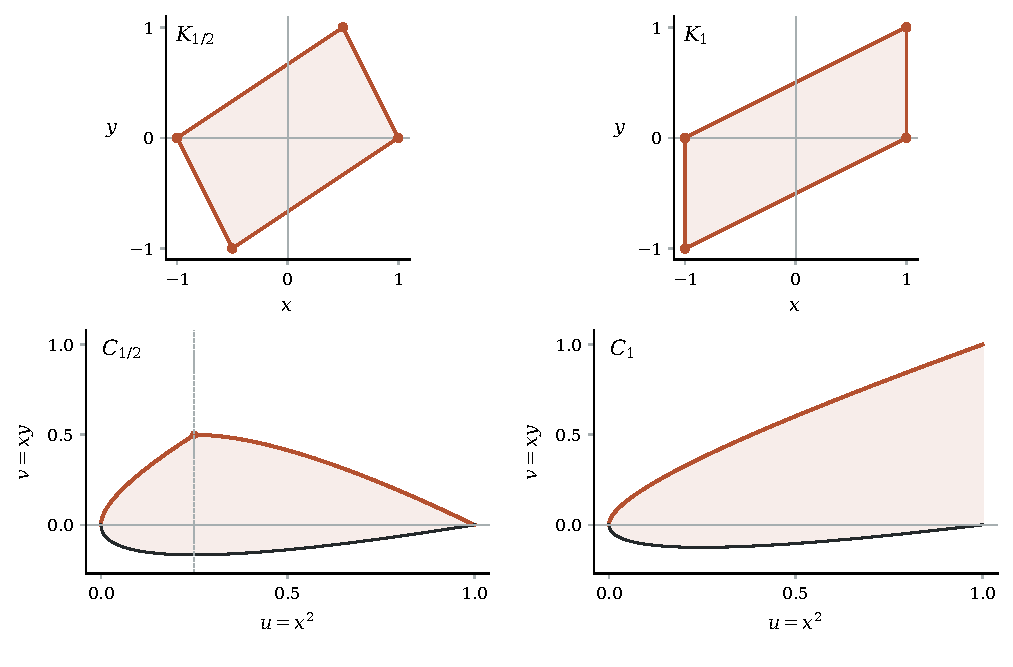
\includegraphics[width=.90\linewidth]{figures/tent-caps-compact.pdf}
 \caption{A single-tent source and its cap under $(x,y)\mapsto(x^2,xy)$.
 The endpoint $a=1$ is a limit of the tent family and is affine equivalent
 to the parabolic cap producing the sharp constant five.}
 \label{fig:tent-caps}
\end{figure}

\subsection{The scalar inequality}
Write $a_0=\sqrt2-1$ and $t=a^2$. Direct integration of the maximizing branches gives
\[
 N(f_a)=\begin{cases}
 \displaystyle\frac{136+24t-64t^2+3(1-t)^2\log((9-t)/(1-t))}{96(1-t)},&0\leq a\leq a_0,\\[6pt]
 \displaystyle\frac{100a^2+120a+100+3(a^2-1)\log((3a-1)/(3-a))}{96},&a_0\leq a<1.
 \end{cases}
\]
The maximizing-branch derivation is supplied below. These formulas imply $N(f_a)<5A(f_a)$ throughout. In the first range,
\[
 5A-N=\frac{8-8t-32t^2-(1-t)^2\log((9-t)/(1-t))}{32(1-t)}>0,
\]
since $t\leq3-2\sqrt2<1/5$ makes the numerator at least $128/25-\log11>0$. In the second range, put $r=(3a-1)/(3-a)\in(0,1)$. Then
\[
 5A-N=\frac{1-a}{32}\big[(1+a)\log r+20(1-a)\big].
\]
The trapezoidal upper estimate for the integral of the convex function $1/x$ gives $-\log r\leq(1-r)(1+1/r)/2$. The bracket is therefore at least
\[
 (1-a)\left[20-\frac{4(a+1)^2}{(3-a)(3a-1)}\right]>0,
\]
because $5(3-a)(3a-1)-(a+1)^2=-16(a^2-3a+1)>0$ for $a_0\leq a<1$.

\begin{theorem}[Sharp planar difference-area bound]
For every origin-symmetric planar convex body $K$,
\[
 \area(\sigma K-\sigma K)\leq5\area(\sigma K).
\]
The constant five cannot be decreased. The same inequality holds for every planar reciprocal body and every affine image of such a body.
\end{theorem}
\begin{proof}
Combine the one-parameter reduction with the scalar inequalities. For sharpness take $K_\epsilon=[-1,1]\times[-\epsilon,\epsilon]$. After the affine normalization $(u,v)\mapsto(u,v/(2\epsilon))$, its squared image tends to $\{0\leq u\leq1,|v|\leq\sqrt u\}$, whose difference area is five times its area.
\end{proof}
The Chaidez--Tanny reversibilization argument consequently gives the explicit bound $c_{\rm EHZ}(X)^2\leq\frac52\operatorname{vol}_4(X)$ for $I$-invariant convex bodies in four dimensions. Sharpness of the standalone planar bound does not establish optimality of this symplectic constant.

\subsection{Deriving the two exact area formulas}
Here are finite formulas verifying the stated exact areas. For $\alpha\in(-1,1)$ set
\[
 p_\alpha(r)=\frac{1+\alpha+(1-\alpha)/r}{4},\quad
 q_\alpha(r)=\frac{(1+\alpha)r+1-\alpha}{4},\quad
 s_\alpha(r)=p_\alpha(r)^2-q_\alpha(r)^2,
\]
\[
 F_\alpha(r)=\frac{p_\alpha(r)(1-p_\alpha(r))}{1-\alpha}
 +\frac{q_\alpha(r)(1-q_\alpha(r))}{1+\alpha},\qquad
 J_\alpha(R,S)=\int_R^S F_\alpha(r)s_\alpha'(r)\,dr.
\]
These arise by setting $p=\sqrt{u+s}$ and $q=\sqrt u$ in the maxima. Smooth stationarity is $(1+a)/p+(1-a)/q=4$ for $H_+$ and $(1-a)/p+(1+a)/q=4$ for $H_-$. The objective is strictly concave on the smooth pieces; at the kink one checks the two one-sided derivatives. The only further candidate is the endpoint $p=1$.

Put $b=1+a$, $c=1-a$, $q_+=c/(3-a)$, $q_-=b/(3+a)$, and $d=ac/(3a-1)$ when it is used. Define
\[
 \begin{aligned}
 B(q)&=\frac2b\left(\frac{q^3}3-\frac{q^4}4\right),&
 E(q)&=\frac2b\left(\frac{q^3}3+\frac{q^4}4\right),\\
 R(q)&=\frac2c\left(\frac{q^3}3-\frac{q^4}4\right),&
 Q(q)&=a q^2+B(q).
 \end{aligned}
\]
Writing $I_\pm=\int_0^1H_\pm(f_a,s)\,ds$, the exhaustive branch formulas are
{\small
\[
\begin{array}{c|l|l}
\text{range}&I_+&I_-\\\hline
[0,a_0]&J_a(1,q_+)+B(q_+)&J_{-a}(1,q_-)+E(a)+R(q_-)-R(a)\\[2pt]
[a_0,1/2]&J_a(1,q_+)+B(q_+)&J_{-a}(1,(3a-1)/c)+Q(1)-Q(d)+E(a)\\[2pt]
[1/2,1)&Q(a)-Q(d)+J_a(c/(3a-1),q_+)+B(q_+)&Q(1)-Q(a)+E(a)
\end{array}
\]
}
In the first range both maxima start at $p=q=1/2$ and follow stationary arcs until $p=1$. For $H_-$ the remaining endpoint arc crosses $q=a$, explaining its two elementary primitives. In the middle range $H_-$ hits the kink $q=a$ before $p=1$. In the last range $H_-$ starts at this kink, while $H_+$ starts at $p=a$ before reaching its stationary arc. The thresholds are exactly $q_-=a\iff a=a_0$ and $d=a\iff a=1/2$.

For a direct integration check, $F_\alpha s_\alpha'=\sum_{k=-5}^3c_k r^k$, with coefficients
\[
\begin{array}{c|l@{\qquad}c|l}
k&c_k&k&c_k\\\hline
3&(\alpha+1)^3/128&-1&(\alpha^2-1)/64\\
2&-(\alpha+1)^2(3\alpha+1)/128&-2&-(\alpha^3+\alpha^2-\alpha+7)/128\\
1&(\alpha+1)(\alpha^3-\alpha+4)/(64(\alpha-1))&-3&-(\alpha-1)(\alpha^3-\alpha-4)/(64(\alpha+1))\\
0&(\alpha^3-\alpha^2-\alpha-7)/128&-4&(\alpha-1)^2(3\alpha-1)/128\\
&&-5&-(\alpha-1)^3/128
\end{array}
\]
Thus $J$ has the elementary primitive $c_{-1}\log r+\sum_{k\ne-1}c_k r^{k+1}/(k+1)$. Substitution into $N=2(I_++I_-)$ yields the two displayed area formulas; the middle and last ranges simplify to the same expression.


\subsection{Finsler and symplectic consequences}

We give the normalization in the transfer explicitly. For a Finsler metric
$F$ on $\mathbb{RP}^2$, let $\ell(F)$ be its shortest noncontractible
closed-geodesic length, and put
\[
 \mathcal V(F)=\int_{D_F^*\mathbb{RP}^2}\frac{\omega_{\mathrm{can}}^2}{2}.
\]
This is the unnormalized cotangent volume used by Chaidez--Tanny; it is
$\pi$ times the usual normalized Holmes--Thompson area. Let
$\overline F(v)=(F(v)+F(-v))/2$. Its unit codisks are
$(D_x^*F-D_x^*F)/2$, because the support function of this Minkowski average
is the average of the two tangent norms. The sharp planar theorem therefore gives
\[
 \mathcal V(\overline F)\leq\frac54\mathcal V(F)
\]
whenever all the unit codisks of $F$ are affine images of squared bodies.

\begin{corollary}\label{cor:squared-finsler}
For such a Finsler metric on $\mathbb{RP}^2$,
\[
 \ell(F)^2\leq\frac58\mathcal V(F).
\]
\end{corollary}
\begin{proof}
For any noncontractible loop, at least one of its two orientations has
$F$-length at most its $\overline F$-length. Thus
$\ell(F)\leq\ell(\overline F)$. The reversible Ivanov--Pu inequality,
in the normalization above, is
$\ell(\overline F)^2\leq\mathcal V(\overline F)/2$;
see \cite[Theorem~3.7 and Lemma~3.8]{CT2026}. Combine these inequalities.
\end{proof}

\begin{corollary}\label{cor:I-symmetric}
Let $X\subset\mathbb H$ be a full-dimensional convex body invariant
under right multiplication by the quaternion $I$, with the standard
symplectic structure in \cite{CT2026}. Then
\[
 c_{\EHZ}(X)^2\leq\frac52\Vol_4(X),\qquad
 \rho(X)\leq\frac54.
\]
\end{corollary}
\begin{proof}
First suppose $X$ is smooth and uniformly convex. The quaternionic
construction of Chaidez--Tanny associates a Finsler metric $F$ on
$\mathbb{RP}^2$ whose unit codisks are affine squared bodies. Their
four-sheet contact covering gives
\[
 c_{\EHZ}(X)\leq4\ell(F),\qquad
 \Vol_4(X)=4\mathcal V(F)
\]
(\cite[Theorem~4.4 and equations~(5.2)--(5.3)]{CT2026}). Hence
\[
 c_{\EHZ}(X)^2\leq16\ell(F)^2
 \leq10\mathcal V(F)=\frac52\Vol_4(X).
\]
For arbitrary convex $X$, use smooth uniformly convex approximants with
the same finite symmetry. One obtains them by smoothing the invariant
support function and adding a small Euclidean ball. Hausdorff continuity
of volume and of EHZ capacity passes the bound to $X$, as in
\cite[Remark~5.4]{CT2026}.
\end{proof}

The planar constant five is sharp; neither corollary asserts a sharp
constant for its geometric class. In particular the comparison between a
geodesic and its closed lift, and the compatibility of codisks coming from
one ambient body, may prevent simultaneous equality in the auxiliary
estimates. The corollary gives the explicit constant $\sqrt5/2$ in a setting where
\cite[Theorem~11]{CT2026} supplies an unspecified constant below $\sqrt{3/2}$ ; it does not
establish the Viterbo bound $\rho\leq1$ for $I$-invariant bodies.
